% 论文模板
\documentclass{math-article}

\title{随机计算}
\author{B. R. Gaines}

\begin{document}

\maketitle

\begin{abstract}
    随机计算机是作为学习机研究计划的一部分而发展起来的. 它使用随机序列来表示模拟量，使得可以用简单的数字逻辑电路实现复杂的模拟计算功能. 本文描述了随机计算的基本原理、表示方法、基本运算单元（反相器、乘法器、加法器、积分器）以及随机序列的生成技术，并讨论了随机计算机在自适应控制和模式识别等领域的应用.

    \noindent\textbf{关键词：}\songti\zihao{-4}随机计算，随机计算机，学习机，数字噪声，自适应控制
\end{abstract}

% 导入各章节
\section{Stochastic computing（随机计算）}

by B. R. GAINES

Standard Telecommunication Laboratories

Harlow, Essex, United Kingdom

\section{引言}

随机计算机是作为学习机形式的先进自动控制器之结构、实现与应用研究计划的一部分而发展起来的. \(^{1,2}\) 虽然搜索、辨识、策略形成以及这些活动的整合等算法可以在传统数字计算机上通过仿真进行建立和测试，但尚无硬件支持学习机所需的复杂计算结构. 主要问题是设计一种活性存储元件，其存储值在长期内保持稳定，能够以小的增量进行变化，且其输出可以作为``权重''来乘其他变量. 由于任何实用系统都需要大量此类元件，因此还要求它们体积小、成本低. 传统的模拟积分器和乘法器无法满足稳定性和低成本的要求，而非传统元件如电化学存储器和磁通变换器则不可靠，或需要复杂的外部电路才能使用. \(^{3}\) 半导体集成电路在速度、稳定性、尺寸和成本方面具有优势，因此决定设计一种基于标准门电路和触发器的计算元件，以实现大规模集成.

二进制双向计数器具有增量存储器的特性，但如果增量过小且大小可变，则需要很多位. 然而，若增量过程为随机过程，则可在存储计数中实现``分数增量''. 例如，若增量只需最低有效位值的十分之一，则计数器可以十分之一的概率增加一——这就是随机计算的基本原理：用事件发生的概率来表示模拟量. 这一原理最初在 ADDIE（平滑存储器件）中得到体现，它是一种具有随机输入和输出的平滑与存储器件，用于实现 STeLLA 学习方案，\(^{1}\) 后来扩展形成了一系列能够执行模拟计算机所有正常功能的计算元件家族——这被称为随机计算机. \(^{4}\)

由于本文篇幅所限，只能简要描述一些基本的随机计算元件和配置. 文献 4 讨论了随机计算的理论基础，并描述了一些先前在数据处理中使用随机变量的应用，而文献 5 则描述了随机计算在过程辨识中的应用，包括梯度技术、Bayes 估计与预测以及 Markov 建模.

\section{数值数据的随机表示}\label{stochastic-representation-of-numerical-data}

随机计算机是一种增量计算机或"计数"计算机，其计算涉及无序逻辑电平序列的交互（而非二进制"字"之间的数字运算），这与数字微分分析仪\(^6\)、运算混合计算机\(^7\)以及相位计算机\(^8\)类似. 在所有这些计算机中，数值在存储时表示为二进制字，在计算时表示为时钟序列中 ON 逻辑电平所占比例（或运算计算机和异步 DDA 中的脉冲频率）. 常规计算机中，逻辑电平序列以确定性方式生成，通常呈现规律性模式或重复性. 而在随机计算机中，每个逻辑电平均由统计独立的过程生成，仅该过程的生成概率由待表示的数值决定.

图 1 展示了各类计算机中的典型序列，说明了这种区别：(a) 是同步速率乘法器的输出，或 DDA 中"R 寄存器"的输出，对应于存储量满 $\frac{3}{4}$ 的情况——注意 ON 和 OFF 逻辑电平分布均匀；(b) 是相位计算机中差分

\begin{figure}[htbp]
    \centering
    \begin{tabular}{ll}
        (a) & O I I O I I O I I O I I 速率乘法器输出 \\
        (b) & 差分存储器输出 \\
        (c) & O I O I I I I I O O I I I O \\
        (d) & \\ \\
        (e) & \\ \\
        (f) & 随机序列总体
    \end{tabular}
    \caption{各类增量计算机中的典型计算序列}
\end{figure}

存储器的输出——在一个周期内，所有的 OFF 逻辑电平都出现在 ON 逻辑电平之前，形成 mark/space 调制信号的同步等价形式；(c) 至 (f) 是生成概率为 $\frac{3}{4}$ 的随机序列示例——任何序列[包括 (a) 和 (b)]都可能出现，但在这类序列的大样本中，ON 电平比例服从均值为 $\frac{3}{4}$ 的二项分布.

尽管概率是能够表示模拟数据而无量化误差的连续变量，但该变量无法被精确测量，且会受到估计方差的影响. 比较各类计算机以 $1/N$ 精度承载模拟数据所需的电平数，可见方差对表示效率的影响：

\begin{itemize}
    \item 模拟计算机需要一个连续电平；
    \item 数字计算机需要 $\log_2 \mathbf{kN}$ 个有序二进制电平；
    \item DDA 需要 $\mathbf{kN}$ 个无序二进制电平；以及
    \item 随机计算机需要 $\mathbf{kN}^2$ 个无序二进制电平；
\end{itemize}

其中 $\mathbf{k} > 1$ 是表示舍入误差或方差影响的常数，例如 $\mathbf{k} = 10$. 随机计算机的 $\mathbf{N}^2$ 项源于：估计生成概率的期望误差随所采样序列长度的平方根而减小.

尽管从 $1 : \log_2\mathbf{N} : \mathbf{N} : \mathbf{N}^2$ 这一进展来看，随机计算机在数量表示方面效率最低，但随机序列缺乏相干性或规律性，使得可以使用简单的硬件来完成用这种形式表示的数据的复杂计算.

\section{随机计算}

尽管在某些情况下，概率的 $[0, 1]$ 范围可以直接用于计算，例如 Bayes 估计与预测，但通常需要通过缩放和原点平移将模拟变量映射到该范围. 已研究了许多映射方法，但本文考虑的两种映射具有特殊意义，因其产生的计算类似于传统模拟计算机的计算. 这两种映射是：

\begin{enumerate}
    \item[(i)] 单线对称表示. 给定一个量 $\mathbf{E}$，其范围为 $-\mathbf{V} \leqslant \mathbf{E} \leqslant \mathbf{V}$，用一个生成概率为 $\mathfrak{p}$ 的序列来表示它，使得：
\end{enumerate}

\[
p (O N) = \frac {1}{2} E / V + \frac {1}{2} \tag {1}
\]

因此，最大正量由始终为 ON 的逻辑电平表示，最大负量由始终为 OFF 的逻辑电平表示，而零量则由 ON 和 OFF 概率相等的随机序列表示.

\begin{enumerate}
    \item[(ii)] 双线对称表示. 第一种表示存在一个缺点，即零量是以最大方差表示的. 当需要区分接近零的值时，最好使用双线随机表示. 设量 $\mathbf{E}$ 的范围为 $-\mathbf{V} \leqslant \mathbf{E} \leqslant \mathbf{V}$，用两条线上的序列表示，即 UP 线和 DOWN 线，使得：
\end{enumerate}

\[
p (U P = O N) = \left\{ \begin{array}{l l} E / V & \text {i f} E > 0 \\ 0 & \text {i f} E \leqslant 0 \end{array} \right. \tag {2}
\]

\[
p (\text {D O W N} = \text {O N}) = \left\{ \begin{array}{l l} - E / V & \text {i f} E <   0 \\ 0 & \text {i f} E \geqslant 0 \end{array} \right. \tag {3}
\]

这些方程给出了一种最小方差表示，但这不一定在计算过程中保持，而双线对称表示的最一般形式来自逆方程：

\[
\mathrm {E} / \mathrm {V} = \mathrm {p} (\mathrm {U P} = \mathrm {O N}) - \mathrm {p} (\mathrm {D O W N} = \mathrm {O N}) \tag {4}
\]

下面描述用于执行完整模拟计算功能（包括反相、乘法、加法、积分等）的随机计算元件，这些元件使用对随机序列进行操作的同步逻辑元件.

\section{随机反相器、乘法器和隔离器}

要将表示形式 (ii) 中的量乘以 $-1$，只需交换 UP 和 DOWN 线路. 在表示形式 (i) 中，逻辑反相器（其输出为其输入的补）执行相同的功能. 考虑其输出为 ON 的概率 $\mathbf{p}^{\prime}$ 与其输入为 ON 的概率 p 之间的关系. 即

\[
p^{\prime} = 1 - p \tag{5}
\]

由公式 (1)，这些概率与它们所表示的量之间的关系为：

\[
\begin{array}{l}
p = \frac{1}{2} E / V + \frac{1}{2} \\
p^{\prime} = \frac{1}{2} E^{\prime} / V + \frac{1}{2}
\end{array}
\]

因此

\[
\mathbf{E}^{\prime} = -\mathbf{E} \tag{8}
\]

将一个量与另一个量相乘可以通过表示形式 (i) 中的反相异或门以及表示形式 (ii) 中的一对类似门来实现. 图 3(i) 和 3(ii) 分别展示了这些随机乘法器在 NAND 逻辑中的实现.

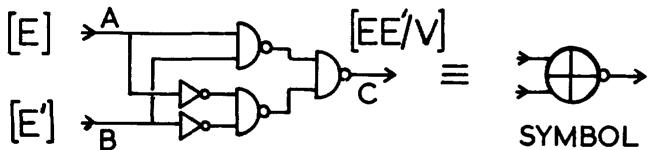
\includegraphics[width=0.6\textwidth, height=7cm, keepaspectratio]{images/006cd21d90ed91a778330bc2c7410063641a619aaeebcfebb6a1829dec084b21.jpg}\\
(i) $C = A.B \vee \overline{A}.\overline{B}$

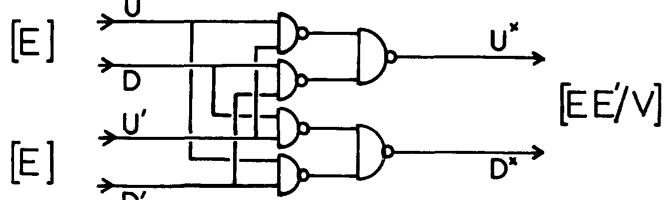
\includegraphics[width=0.6\textwidth, height=7cm, keepaspectratio]{images/87b5233b7b2642581fc555b9961d8e8aaeb4f0652acf86b532de3129ae1a8def.jpg}\\
$U^* = U.U^{\prime} \vee D.D^{\prime}$ (ii)\\
$D^* = U.D^{\prime} \vee D.U^{\prime}$

图 3---随机乘法器

检验图 3 中门的输入和输出概率之间的关系，可确认确实执行了乘法运算. 对于 3(i)：

\[
\begin{array}{l}
\mathrm{p}(\mathrm{C}) = \mathrm{p}(\mathrm{A}) \mathrm{p}(\mathrm{B}) + (1 - \mathrm{p}(\mathrm{A})) (1 - \mathrm{p}(\mathrm{B})) \\
\text{由公式 (1)：}
\end{array} \tag{9}
\]

\[
p(A) = \frac{1}{2} E / V + \frac{1}{2} \tag{10}
\]

\[
p(B) = \frac{1}{2} E^{\prime} / V + \frac{1}{2} \tag{11}
\]

因此：

\[
p(C) = \frac{1}{2} \left(E E^{\prime} / V\right) / V + \frac{1}{2} \tag{12}
\]

这是对 $E$ 与 $\mathbf{E}^{\prime}$ 的归一化乘法. 对于 3(ii)，将公式 (4) 代入以下关系式，可得类似结果：

\[
\begin{array}{l}
p(U^*) = p(U) p\left(U^{\prime}\right) + p(D) p\left(D^{\prime}\right) - \\
\mathrm{p}\left(\mathrm{U} \cdot \mathrm{U}^{\prime} \cdot \mathrm{D} \cdot \mathrm{D}^{\prime}\right)
\end{array} \tag{13}
\]

以及：

\[
\begin{array}{rl}
\mathrm{p}\left(\mathrm{D}^{*}\right) & = \mathrm{p}(\mathrm{U}) \mathrm{p}\left(\mathrm{D}^{\prime}\right) + \mathrm{p}(\mathrm{D}) \mathrm{p}\left(\mathrm{U}^{\prime}\right) - \\
& \mathrm{p}\left(\mathrm{U} \cdot \mathrm{U}^{\prime} \cdot \mathrm{D} \cdot \mathrm{D}^{\prime}\right)
\end{array} \tag{14}
\]

以随机乘法器作平方器时，揭示了一个重要现象. 例如，仅将图 3(i) 中门的输入短接是不够的，因其输出将始终为 ON. 出现这一困难的原因在于，推导上述公式 (9) 时假设随机输入序列是统计独立的. 幸运的是，可通过将序列延迟一个事件来获得随机序列（实际上是 Bernoulli 序列）的独立复制. 图 (4) 展示了如何使用图 3(i) 的乘法器和一个用作延迟的触发器来构造一个平方器. 类似地，图 3(ii) 的乘法器可通过将 U 和 D 的延迟复制分别馈送到 $U^{\prime}$ 和 $D^{\prime}$ 来用作平方器. 以这种方式使用的触发器充当随机``隔离器''，不执行计算，但统计上隔离两条互相关的线路.

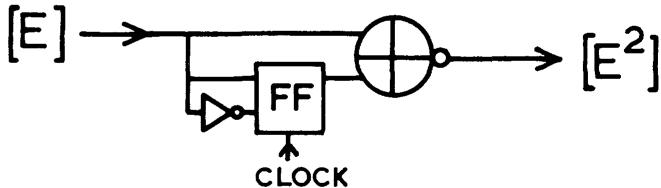
\includegraphics[width=0.6\textwidth, height=7cm, keepaspectratio]{images/879c30ec366d098fb9151a70770fff6be90fbcfc2bb7c014fac61ebfe974c207.jpg}\\
图 4---随机平方器

\section{随机加法器和积分器}

在了解了如何通过简单门电路轻松实现求反和乘法之后，人们或许会想当然地认为类似的门电路也可用来实现加法. 然而事实并非如此，必须引入随机逻辑元件来对两个随机序列所表示的量进行求和. 例如，考虑表示 (i) 中的两个随机序列，一个表示最大正量因此始终为 ON，另一个表示最大负量因此始终为 OFF. 这两个量之和为零，其表示是一个 ON 和 OFF 概率相等的随机序列. 无法从具有恒定输入的确定性门电路获得概率性输出，因此必须在随机计算机的求和门电路中内置随机行为.

随机加法器可被视为一种开关，它在时钟脉冲时随机选择一条输入线并将其连接到输出端. 输出线则表示输入线所表示的量的和，根据选择特定输入线的概率进行加权. 随机选择由内部生成的随机序列执行，这些序列通过采样由高带宽噪声源触发的触发器，或从中央伪随机移位寄存器的延迟序列获得. 称这些序列为「数字噪声」.

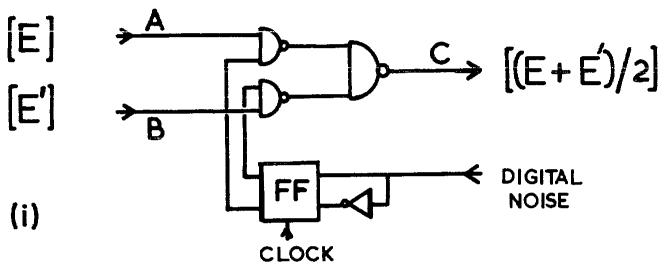
\includegraphics[width=0.6\textwidth, height=7cm, keepaspectratio]{images/5dc94beb4b8df8ffaa7d0969fa68d04c38fcfc80f4ba37c1f9038e19a6ebcd10.jpg}

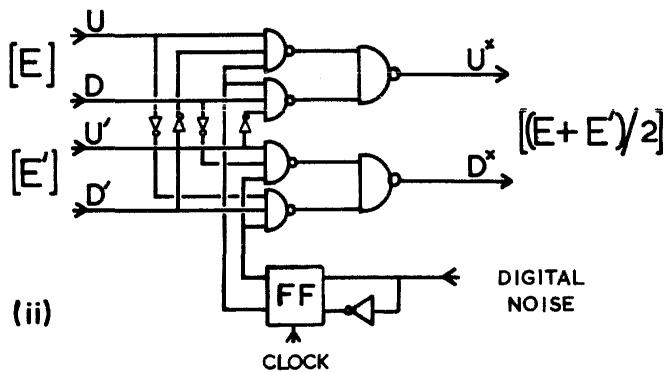
\includegraphics[width=0.6\textwidth, height=7cm, keepaspectratio]{images/bbed31d4771fbde4344e3774419967d9fc2a2d9dec06eb85f04836fb0862bd0f.jpg}\\
Figure 5---随机加法器

表示 (i) 和 (ii) 中用于两个输入的随机加法器分别如图 5(i) 和 5(ii) 所示. 图 5(ii) 中输入之间的交叉耦合降低了输出的方差. 检查图 5 中门电路的输入和输出概率之间的关系，可确认确实执行了加法. 对于 5(i)，假设数字噪声对称分布：

\[
\mathbf {p} (\mathrm {C}) = \frac {1}{2} \mathbf {p} (\mathrm {A}) + \frac {1}{2} \mathbf {p} (\mathrm {B}) \tag {15}
\]

因此，根据公式 (10) 和 (11)：---

\[
\mathbf {p} (\mathbf {C}) = \frac {1}{2} \left(\frac {1}{2} \left(\mathrm {E} + \mathrm {E} ^ {\prime}\right)\right) / \mathrm {V} + \frac {1}{2} \tag {16}
\]

这是 $\mathbf{E}$ 和 $\mathbf{E}^{\prime}$ 的归一化求和. 将公式 (4) 代入以下关系式，可为 5(ii) 获得类似结果：

\[
\begin{array}{l} p (U ^ {x}) = \frac {1}{2} p (U) (1 - p (D ^ {\prime})) + \frac {1}{2} p (U ^ {\prime}) \\ (1 - \mathbf {p} (D)) \tag {17} \\ \end{array}
\]

\[
\begin{array}{l} p \left(\mathrm {D} ^ {\mathrm {x}}\right) = 1 / 2 p (\mathrm {D}) (1 - p \left(\mathrm {U} ^ {\prime}\right)) + 1 / 2 p \left(\mathrm {D} ^ {\prime}\right) \\ (1 - p (U)) \tag {18} \\ \end{array}
\]

随机积分器、ADDIE 和接口

随机计算机中的基本积分器是可逆计数器---若它有 $\mathbf{N} + 1$ 个状态，则当其处于第 k 个状态时，积分的值为：

\[
f = (2 k / N - 1) V \tag {19}
\]

若要在进一步的计算中使用这个量，必须将其作为随机序列提供，这可通过将计数器中的二进制数与均匀分布的数字随机数（从中央伪随机移位寄存器或采样循环计数器获得）进行比较来生成. 在表示 (i) 中，若存储计数大于随机数，则积分器输出线为 ON. 在表示 (ii) 中，存储计数被视为二进制补码表示的数，其幅度与随机数比较，其符号与比较结果一起决定 UP 或 DOWN 输出线应为 ON.

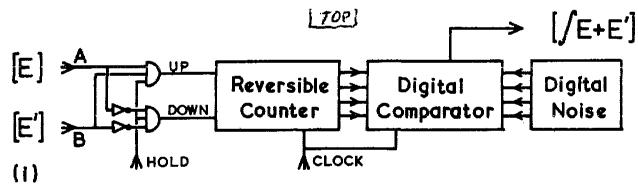
\includegraphics[width=0.6\textwidth, height=7cm, keepaspectratio]{images/007a2e69d1cdef90fea0e84ae3f7f572dd8e39f1a4ab896936ec0d15e7299444.jpg}

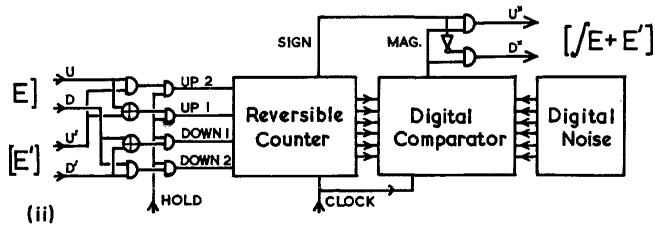
\includegraphics[width=0.6\textwidth, height=7cm, keepaspectratio]{images/16ec18facc1380b8aa3b7486b50e51a35cfe61959404adde710f746e5c26117d.jpg}\\
Figure 6---随机积分器

图 6 显示了每种表示的两个输入随机积分器，其输出线如上所述，并在计数器输入端设置门电路以形成输入线所表示量的和（不需要随机求和，因为用于表示和的线数大于用于表示每个输入的线数）. 积分器输入端的 HOLD 线决定它们处于积分模式还是保持模式，并且

正常的积分器符号用于整体设备，如图 7 所示.

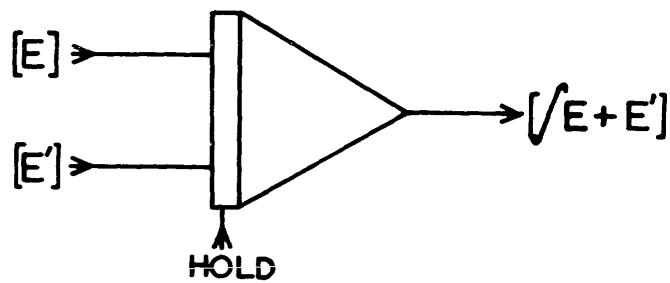
\includegraphics[width=0.6\textwidth, height=7cm, keepaspectratio]{images/75a79ae91e0524d8a4a085913776e7eb6366e36494880280cd89973d641fcbec.jpg}\\
Figure 7---积分器符号

检查每个时钟脉冲时计数器的预期增量 $\delta$，可确认确实执行了积分. 对于 6(i)：

\[
\begin{array}{l} \delta = \frac {2 \mathrm {V}}{\mathrm {N}} [ \mathrm {p} (\mathrm {A}) \mathrm {p} (\mathrm {B}) - (1 - \mathrm {p} (\mathrm {A}) (1 - \mathrm {p} (\mathrm {B})) ] (20) \\ = \left(\mathrm {E} + \mathrm {E} ^ {\prime}\right) / \mathrm {N} (21) \\ \end{array}
\]

代入公式 (10) 和 (11)，这等效于一个具有时间常数的积分器：

\[
\mathrm {T} = \mathrm {N} / \mathrm {f} \tag {22}
\]

其中 $f$ 是时钟频率. 将公式 (4) 代入以下关系式，可为 6(ii) 获得类似结果：

\[
\begin{array}{l} \delta = \frac {2 \mathrm {V}}{\mathrm {N}} [ 2 \mathrm {p} (\mathrm {U}) \mathrm {p} (\mathrm {U} ^ {\prime}) + \mathrm {p} (\mathrm {U}) (1 - \mathrm {p} (\mathrm {U} ^ {\prime})) + \mathrm {p} (\mathrm {U} ^ {\prime}) \\ (1 - p (U)) - 2 p (D) p \left(D ^ {\prime}\right) - p (D) (1 - p \left(D ^ {\prime}\right)) \\ - p (D ^ {\prime}) (1 - p (D)) ] (23) \\ = \frac {2 V}{N} [ p (U) - p (D) + p \left(U ^ {\prime}\right) - p \left(D ^ {\prime}\right) ] (24) \\ = 2 \left(\mathrm {E} + \mathrm {E} ^ {\prime}\right) / \mathrm {N} (25) \\ \end{array}
\]

这等效于一个具有时间常数的积分：

\[
\mathrm {T} = \mathrm {N} / 2 \mathrm {f} \tag {26}
\]

其中 $f$ 是时钟频率.

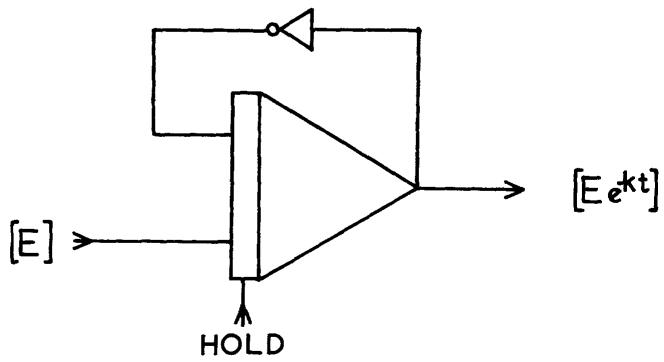
\includegraphics[width=0.6\textwidth, height=7cm, keepaspectratio]{images/0cdd3c8d1eaae3776bcc0f46af2de49d369be1891bdabfe0bafb2233add619e1.jpg}\\
Figure 8-ADDIE

图 8 所示的具有单位反馈的积分器称为 ADDIE，它执行对其输入所表示的量进行指数平均的重要功能. 就所表示的量而言，它可以被视为传递函数：$1 / (s + 1)$. 就随机序列而言

可证，存储器中的分数计数趋于输入线在时钟脉冲时为 ON 的概率的无偏估计（对于如图 8 所示连接的图 6(i) 积分器）. 即，对于处于 $k^{\prime}$ 状态的 $\mathbf{N} + 1$ 状态存储器：

\[
\hat {\mathbf {p}} (\text {I N P U T} = \mathrm {O N}) = \mathrm {k} / \mathrm {N} \tag {27}
\]

估计时间为 N 个时钟脉冲数量级，最终方差为：

\[
\sigma^ {2} (\hat {\mathfrak {p}}) = \mathrm {p} (1 - \mathrm {p}) / \mathrm {N} \tag {28}
\]

因此，随机计算机中由概率线性表示的任何量均可通过使用具有足够多状态的 ADDIE 以任意所需精度读出，但状态越多，平滑的时间常数越长，计算机的带宽越低. 由于积分器中计数的分布是二项分布，因此对于大 N 近似正态分布，随机计算机内的变量可被视为被 Gaussian 噪声退化，其功率随计算机所需带宽成比例增加.

积分器或 ADDIE 构成随机计算机的自然输出接口. HOLD 线为 OFF 的积分器也构成数字或模拟数据的输入接口，因为可以直接将二进制数传送到计数器中以生成随机输出序列，并且可以通过将模拟量与由驱动数模转换器的循环计数器生成的标准斜坡进行比较来将其转换为二进制形式. 类似地，若与乘法器耦合，积分器可用于保持常数，从而充当「电位器」. 可通过在存储计数和随机输出之间施加适当的非线性关系来实现任意函数关系. 例如，一个积分器当其输出在计数值等于或高于中值时为 ON，在低于中值时为 OFF [表示 (i) 中]，近似于开关函数.

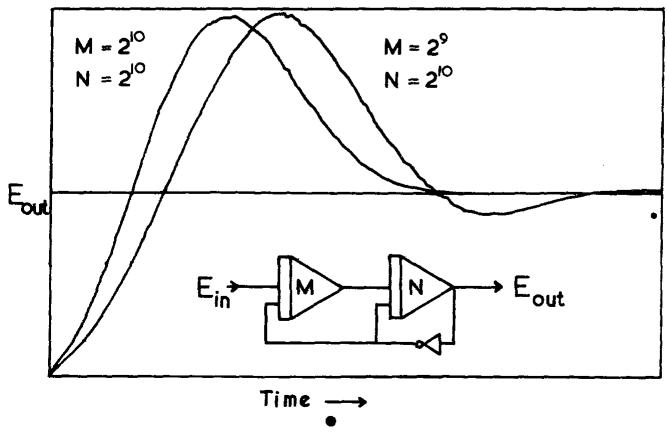
\includegraphics[width=0.6\textwidth, height=7cm, keepaspectratio]{images/ed44eb7f2d5c2d711785ea2583ca50f72f6b7b5057c9faad71f2c99fcd1d2e5f.jpg}\\
Figure 9---随机二阶传递函数---对位置和速度单位阶跃的响应

通过将积分器级联连接并设置适当的反馈回路，可以实现比 ADDIE 更高阶的平滑. 图 9 的插图显示了使用表示 (i) 中两个随机积分器的稳定二阶随机传递函数. 若第一个积分器有 $\mathbf{M} + 1$ 个状态，第二个有 $\mathbf{N} + 1$ 个状态，则实现的变换为：

\[
\frac {\mathrm {M N}}{\mathrm {f} ^ {2}} \mathrm {E} _ {\text {o u t}} + \frac {\mathrm {M}}{\mathrm {f}} \mathrm {E} _ {\text {o u t}} + \mathrm {E} _ {\text {o u t}} = \mathrm {E} _ {\text {i n}} \tag {29}
\]

其中 $f$ 是时钟频率. 因此无阻尼自然频率为：

\[
\mathrm {f} _ {\mathrm {n}} = \frac {\mathrm {f}}{2 \Pi (\mathrm {M N}) ^ {1 / 2}} \tag {30}
\]

阻尼比为：

\[
\Sigma = 1 / 2 (\mathrm {M} / \mathrm {N}) ^ {1 / 2} \tag {31}
\]

对位置和速度单位阶跃的响应如图 9 所示，对应两种条件：$\mathbf{M} = 2^{10}$，$\mathbf{N} = 2^{10}$ 和 $\mathbf{M} = 2^{9}$，$\mathbf{N} = 2^{10}$. 这些是在 STL 的 Mark I 随机计算机上获得的.

\section{随机序列的生成}

构建随机计算机的核心问题在于生成多个随机序列（每个积分器需要K个，K为积分器计数器中的触发器数量），这些序列既不能互相关也不能自相关，且具有已知且稳定的生成概率. 这可归结为需要多个统计独立的序列，每个序列的生成概率为$\frac{1}{2}$，因任何概率均可表示为二进制小数，并通过适当选通一组等概率为 ON 或 OFF 的线路来实现任意所需精度. 例如，图 10 展示了一种通过采样来自噪声源的快速翻转触发器来生成生成概率为$\frac{1}{2}$的随机序列的技术：随后的 NAND 门将其中两个序列转换为生成概率为$\frac{3}{4}$的序列. 这可通过以下关系式加以验证：

\[
\mathrm {p} (\mathrm {C}) = (1 - \mathrm {p} (\mathrm {A})) + \mathrm {p} (\mathrm {A}) \mathrm {p} (\mathrm {B}) = 3 / 4 \tag {32}
\]

如图 10 所示，生成数字噪声的方法颇具吸引力，因放射性或光子发射源可直接与半导体器件耦合以形成随机脉冲发生器. 但其缺点在于，若要在随机计算机中使用高时钟频率，则必须在$\mathbf{F}\mathbf{F}_1$和$\mathbf{F}\mathbf{F}_1^{\prime}$中实现非常高的翻转速率，并通过$\mathbf{F}\mathbf{F}_2$和$\mathbf{F}\mathbf{F}_2^{\prime}$中的非常窄的选通脉冲进行采样.

Mark I 型随机计算机有六个十位积分器，每个积分器都有其独立的内部数字噪声源，由在高速时钟频率下循环的十位计数器组成. 这些计数器以低得多的非谐波时钟频率进行采样，以产生有效的随机输出. 这种安排并不实用，因采样频率必须非常低（500周），以至于计算机的整体带宽仅为0.1周！然而，作为一种实验工具，它使我们能够检验图 9 所示配置等行为，而这些行为在理论上难以确定.

\begin{figure}[htbp]
    \centering
    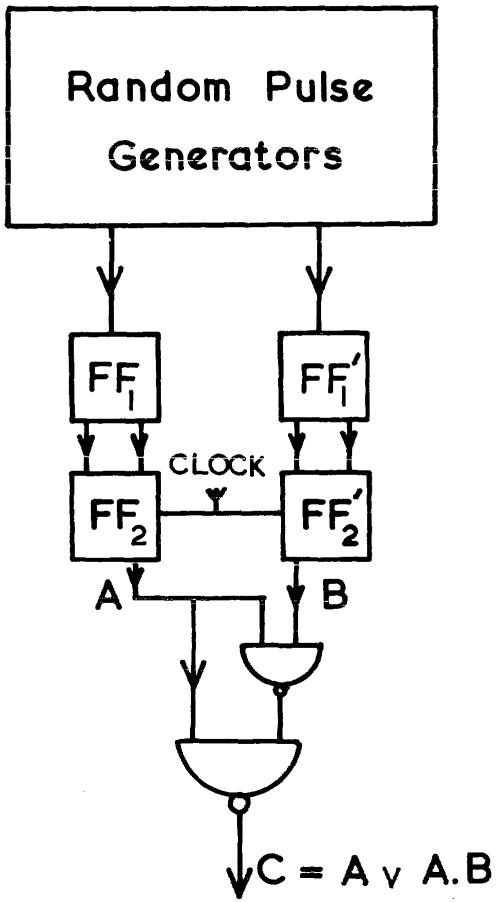
\includegraphics[width=0.6\textwidth, height=7cm, keepaspectratio]{images/86d4c25b150612ffb31e1017b90576a3917bdbf1872594a8388c5304573a1f6b.jpg}
    \caption{随机序列的生成$(p = 3/4)$}
\end{figure}

目前正在建造中的 Mark II 型随机计算机采用了完全不同的技术，既减小了体积和成本，又将时钟频率提高到了1兆周. 采用一个单一的中央伪随机移位寄存器来为所有计算单元生成随机序列. 通过适当的异或门选通移位寄存器输出，可以获得移位寄存器本身序列的延迟副本，从而为每个单元提供不同的序列. 图 11 展示了这样一种生成器，它使用43个触发器，能够在无交叉重复的情况下为一百个16位积分器提供一小时的随机序列.

\begin{figure}[htbp]
    \centering
    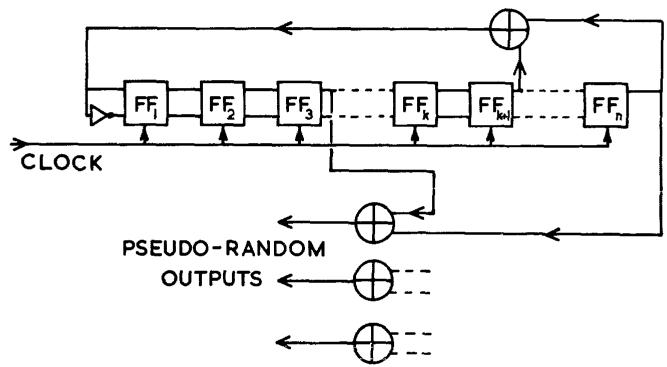
\includegraphics[width=0.6\textwidth, height=7cm, keepaspectratio]{images/e461dd2b34742f61ee15e7f93e5f386678fa36ebbf7e38c1db4fface1c924d3e.jpg}
    \caption{中央伪随机生成器}
\end{figure}

Mark II 型计算机的积分器采用串行运算，因此可以使用移位寄存器实现计数器，并使用少得多的门电路实现比较器. 通过这种方式，现在可以用仅六个双列直插式封装来制造一个十六位随机积分器. 移位寄存器中的16兆周时钟频率在随机计算机中产生1兆周的时钟频率，现在可以实现约100周的相当可观的带宽.

\section{随机计算机的应用}

随机计算机是为解决自动控制领域的问题而开发的，其直接应用主要体现在自适应控制和自适应滤波领域. 用于过程辨识和在线优化的梯度技术是最简单的例子，这类强大的控制方法由于缺乏必要的硬件支持而未能得到充分应用. 使用传统计算机进行直接数字控制对于小型设备来说并不实用，而传统模拟计算机则因需要大量乘法器而成本高昂. 已有研究提出\(^{12}\)采用双电平或极性重合乘法\(^{10,11}\)作为一种利用数字集成电路廉价可靠地实现梯度技术的方法；然而，一项对最速下降计算中六种乘法技术的比较研究表明，在相同收敛时间下，极性重合乘法和继电器乘法产生的参数估计方差远大于等效的随机计算配置.\(^{5}\) 在这一特定计算中，随机乘法器可视为统计线性化\(^{13,14}\)的极性重合乘法器，而向输入信号添加锯齿波抖动以实现这种线性化的方法\(^{11,15,16}\)可以看作是一种获取伪随机序列的技术.

基于条件概率 Bayes 逆的最大似然预测是许多用于控制和模式识别的"学习机"的基础，但估计和预测的方程难以用传统计算元件实现，因此需要使用存储程序数字计算机来进行这项技术的实验. 然而，使用 ADDIE 的三输入变体，归一化似然比的估计和基于它们的预测都变得非常简单，只需很少的硬件即可实现.\(^{5}\)

随机计算在硬件经济性方面的理论基础在于 Rabin\(^{17}\) 和 Paz\(^{18}\) 的一个定理，该定理指出随机（或概率）自动机等价于一个通常具有更多状态的确定性自动机. 这一现象的一个直接实际例子可以在自适应阈值逻辑中找到，该逻辑被用于诸如 Perceptron\(^{19}\) 或 Adaline\(^{20}\) 之类的模式分类器中. 具有离散权重的自适应阈值逻辑元件在 Novikoff 条件\(^{21}\) 下不一定收敛，即使权重可以取到能实现线性可分的值，而等效的随机元件则可以在相同条件下收敛.\(^{5}\)

对这种差异的形象解释是：在具有连续权重的自适应阈值逻辑中，沿最速下降方向前进的路径在权重离散化后无法精确实现，此时存在多个"近似最速下降"的方向. 确定性逻辑必须"选择"其中一个方向，若选"错"了，可能会陷入错误决策的循环，而随机逻辑则以一定概率选择任意可能的下降方向，最终必定会选择正确的方向.

\section{结论}\label{conclusion}

计算机的主要性能指标包括可解决问题的规模和范围、求解的速度和精度，以及计算机的物理尺寸、可靠性和成本. 这些指标之间存在强烈的相互制约关系，不太可能有一种计算机形式在所有指标上都达到最优. 复杂过程的辨识与仿真，以及多变量控制系统的实现，需要大量的计算元件（如乘法器、加法器和积分器）同时工作且成本低廉. 然而，这些元件并不需要快速或精确地计算解，因在经济和化学过程的仿真中，10 cs 的带宽和 1\% 的总体精度已经足够，而在存在反馈的控制系统中，10\% 的计算精度可能就已充足. 在这些情况下，用数字计算机的精度和模拟计算机的速度来换取随机计算机的经济性是较为有利的.

\section{致谢}\label{acknowledgments}

感谢 J. H. Andreae 博士（现就职于新西兰基督城坎特伯雷大学）就学习机和计算机问题与我进行的长久讨论，以及对本文稿的批评意见；感谢 P. L. Joyce 先生构建了第一台随机计算机并获得了图 9 的实验结果；感谢 S.T.L. 允许发表本文.

\section{参考文献}\label{references}

1 J. H. ANDREAE Learning machines in Encyclopaedia of Information,
Linguistics and Control (Pergamon Press, to be published)\\
2 B. R. GAINES and J. H. ANDREAE A learning machine in the context of
the general control problem Proceedings of the 3rd Congress of IFAC
1966\\
3 G. NAGY A survey of analog memory devices IEEE Trans. Electron. Comp.
12 388 1963\\
4 B. R. GAINES Stochastic computers in Encyclopaedia of Information,
Linguistics and Control Pergamon Press, to be published\\
5 B. R. GAINES Techniques of identification with the stochastic computer
Proc. IFAC Symp. Problems of Identification 1967\\
6 F. V. MAYOROV and Y. CHU Digital differential analysers IIiffe Books,
London 1964\\
7 H. SCHMID ``An operational hybrid computing system IEEE Trans.
Electron Comp. 12 715 1963\\
8 B. R. GAINES and P. L. JOYCE Phase computers 5th AICA Congress 1967\\
9 W. W. PETERSON Error correcting codes MIT Press \& Wiley, New York
1961\\
10 C. L. BECKER and J. V. WAIT Two-level correlation on an analog
computer IRE Trans. Electron Comp. 10 752 1961

11 B. P. TH. VELTMAN and A. van den BOS The applicability of the relay
correlator and the polarity coincidence correlator in automatic control
Proc. 2nd Congress IFAC 1963\\
12 P. EYKHOFF, P. M. van der GRINTEN, H. KWAKERNAAK, B. P. TH. VELTMAN
Systems modelling and identification Survey Paper 3rd Congress of IFAC
1966\\
13 O. I. ELGERD High frequency signal injection: a means of changing the
transfer characteristics of nonlinear elements WESCON 1962\\
14 A. A. PERVOZANSKII Random processes in nonlinear control Academic
Press, New York 1965\\
15 P. JESPERS, P. T. CHU, and A. FETTWEIS A new method to compute
correlation functions Proc. Int. Symp. Inf. Theo. 1962\\
16 G. A. KORN Random-process simulation and measurement McGraw Hill,
Inc.~1966\\
17 M. O. RABIN Probabilistic automata Inf. \& Contr. 6 230 1963\\
18 A. PAZ Some aspects of probabilistic automata Inf. \& Contr. 9 26
1966\\
19 F. ROSENBLATT A model for experimental storage in neural networks in
Computer and Information Sciences Spartan Books, Washington, D.C. 1964\\
20 B. WIDROW and F. W. SMITH Pattern-recognizing control systems in
Computer and Information Sciences Spartan Books, Washington, D.C. 1964\\
21 A. NOVIKOFF Convergence proofs for perceptrons in Mathematical Theory
of Automata Polytechnic Press, Brooklyn \& Wiley Interscience 1963


\end{document}
